% This file is part of the Open Source project 'proTironeComputatri'
% (c) 2025 Karsten Reincke (https://github.com/pro-tirone-computatri/protico.ltx)
% It is distributed under the terms of the creative commons license
% CC-BY-4.0 (= https://creativecommons.org/licenses/by/4.0/)


\documentclass[]{beamer}

% design beamer:
% --------------
%\usetheme{EastLansing}
\usetheme{Madrid}
%\usetheme{Boadilla}
%\usetheme{Berkeley}
\usecolortheme{spruce}


% customize your presentation
% ---------------------------
% set paths:

\def\imgGl{../../../img.gl/}
\def\bibGl{../../../bib.gl}
\def\cfgGl{../../../cfg.gl/}
\def\imgLf{../../img.lf}
\def\cfgLf{../../cfg.lf}

% language:
\usepackage[utf8]{inputenc}
\usepackage[english,ngerman]{babel}

\usepackage[backend=biber,style=authortitle-dw,sortlocale=auto,]{biblatex}
\input{\cfgGl/inc.cfg-biber-de.tex}
\ExecuteBibliographyOptions{annotation=false}
\renewcommand*{\bibfont}{\fontsize{8}{10}\selectfont}
\addbibresource{\bibGl/lit.fachinformatik.bib}

%\input{\cfgGl/inc.cfg-ncl-de.tex} %integrate nomenclature

\usepackage{nameref} %for using label as nameref
%language specific quoting signs
\usepackage[style=german,autostyle=true,]{csquotes}

% language specific hyphenation
\input{\cfgGl/inc.babelhyphenations.tex}

\usepackage{hyperref} % allow to use hypelinks
\hypersetup{bookmarks=true,breaklinks=true,colorlinks=true,citecolor=blue,draft=false}

% design:
\usepackage{microtype} % improve the grey value and the line feed handling
\usepackage[absolute,overlay]{textpos}

\usepackage{multirow,tabularx}
\usepackage{fontawesome}
\usepackage{rotating}
\usepackage[dvipsnames]{xcolor}

\newcommand\tcrotate[1]{\begin{turn}{90}{#1}\end{turn}}

% This file is part of the Open Source project 'proTironeComputatri'
% (c) 2025 Karsten Reincke (https://github.com/pro-tirone-computatri/protico.ltx)
% It is distributed under the terms of the creative commons license
% CC-BY-4.0 (= https://creativecommons.org/licenses/by/4.0/)

\newcommand{\mylogo} % define your logo for beamer 
{
  \setlength{\TPHorizModule}{11pt}
  \setlength{\TPVertModule}{11pt}
   % textblock{}{x,y}: pos(x) = leftUpperCorner + (x * \TPHorizModule), pos(y) = leftUpperCorner - (y * \TPVertModule)
  \begin{textblock}{1}(30,0.1)
   \includegraphics[width=25pt,height=25pt]{\imgGl/logo.png}
  \end{textblock}
}
\logo{ \mylogo }



\addtobeamertemplate{footnote}{\hskip -2em}{}

% title frame
\title{LF11c : Prozessdokumentation} 
\subtitle{für die Ausbildung zur Fachinformatikerin\input{\cfgGl/inc.lfn-zp}}
\institute{GS-LDK}
\author{Karsten Reincke}
\date{\today}

\begin{document}
% in a presentation normally it should not benecessary 
% to include the complete bibliography
%\nocite{*} 
\selectlanguage{ngerman}

\begin{frame}
  \titlepage
\end{frame}

%%%%%%%%%%%%%%%%%%%%%%%%%%%%%%%%%%%%%
% add the other topic snippets here
% This file is part of the Open Source project 'proTironeComputatri'
% (c) 2025 Karsten Reincke (https://github.com/pro-tirone-computatri/protico.ltx)
% It is distributed under the terms of the creative commons license
% CC-BY-4.0 (= https://creativecommons.org/licenses/by/4.0/)

\selectlanguage{ngerman}

{
\usebackgroundtemplate{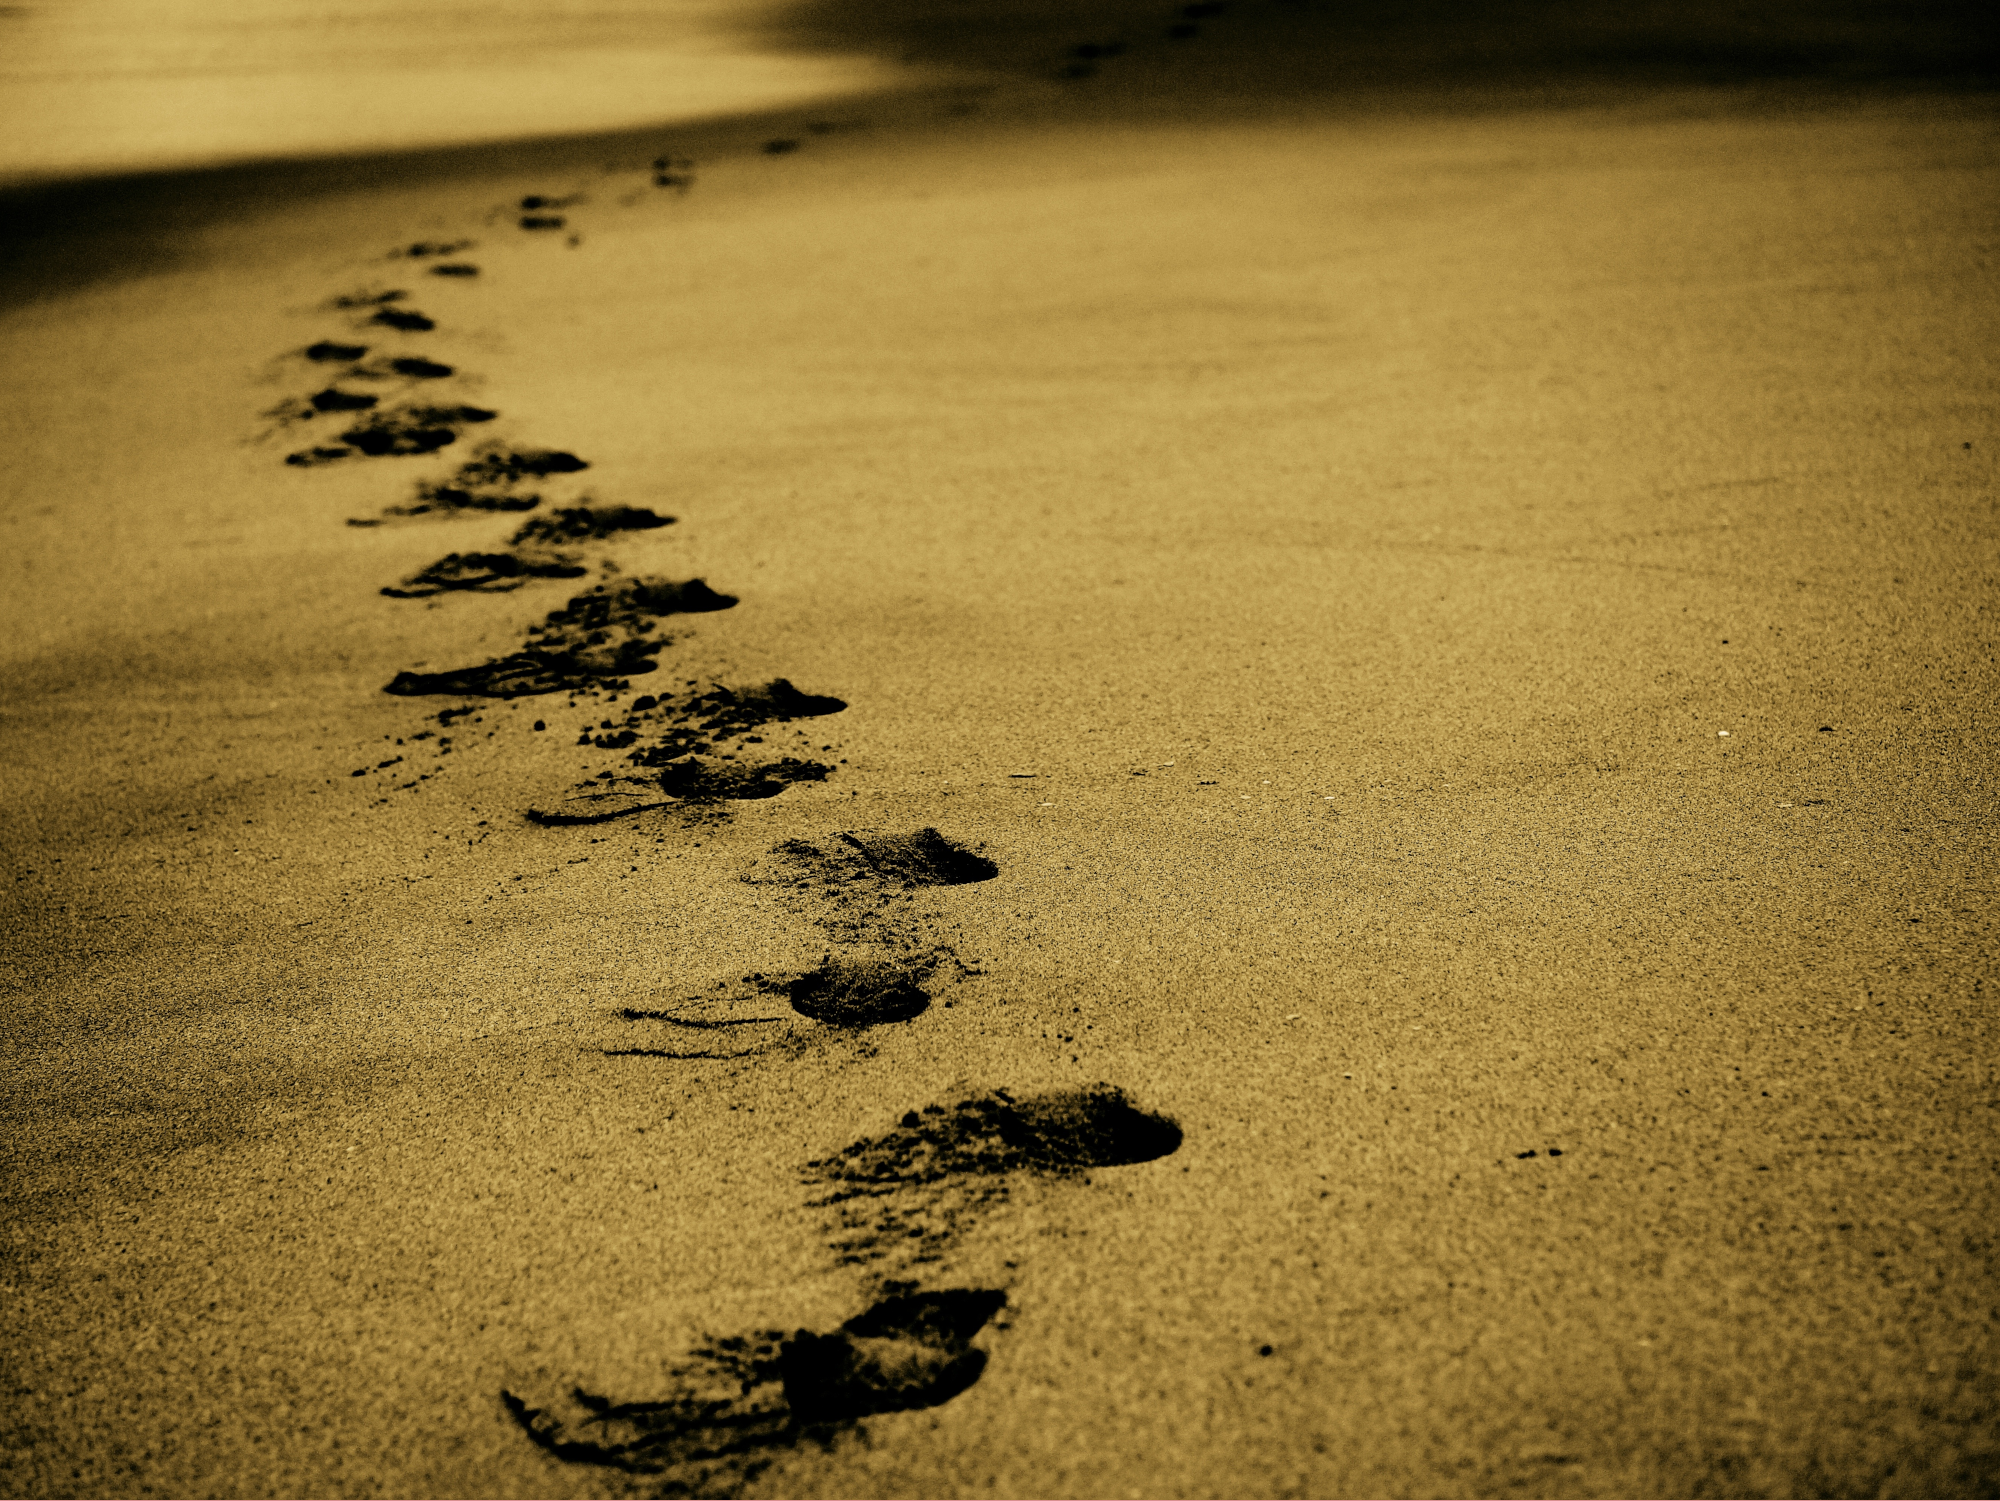
\includegraphics[width=\paperwidth]{\imgLf/beach-steps-725480-pxh.png}}
\begin{frame}  
  \frametitle{LF11c:01:Prozessanalyse}

  \vspace{6cm}
  \begin{flushright}
    \textcolor{white}{Was sind \\
    \textit{Prozesse}?}
  \end{flushright}
\end{frame}
}

\begin{frame}[fragile]
  \frametitle{LF11c:01:Prozessdokumentation:Flow-Chart \& Activity}
  \begin{columns}
    \column{0.5\textwidth}
      \begin{block}{Beispielprozess}
        \begin{verbatim}

cat MIT.dirty.txt |\
   sed 's/  */ /g' |\
   tr -d '\r' |\
   tr '\n' '$' |\
   sed 's/\$\$/\n\n/g' |\
   tr -d '$' |\
   tr 'a' 'a' |\
   sed 's/  */ /g' \
 >> x.txt
        \end{verbatim}
      \end{block}
    \column{0.5\textwidth} 
    \begin{footnotesize}
    \begin{itemize}
      \item \texttt{cat} :- liest Daten aus Datei und gibt sie unverändert nach stdout aus.
      \item \texttt{sed} :- (= Stream-Editor) = liest Daten von \texttt{stdin}, ersetzt das zwischen \texttt{/ /} durch das danach \texttt{/ /} und gibt das Ergebnis nach \texttt{stdout} aus.
      \item \texttt{tr} :- liest Daten von \texttt{stdin}, ersetzt alle Zeichen 'A' durch 'B' bzw. löscht 'A' und schreibt nach \texttt{stdout}
      \item \texttt{>} :- liest von einem IO-Channel (hier \texttt{stdout}) und lenkt die in eine Datei um.
    \end{itemize}
  \end{footnotesize}
  \end{columns}

\end{frame}

{
  \usebackgroundtemplate{\includegraphics[height=\paperheight]{\imgLf/supermarket-898411-pxh.png}}
\begin{frame}[t]
  \frametitle{LF11c:01:Prozessdokumentation:BPMN \& (e)EPK}
  \begin{footnotesize}
    { \bfseries 
  \begin{columns}[t]
    \column{0.5\textwidth}
    \begin{itemize}
      \item Ich bin für's Einkaufen zuständig.
      \item Meine Frau schreibt den Einkaufszettel, schrittweise, wann immer ihr etwas einfällt, manchmal bis zur letzten Minute.
      \item Irgendwann, bevor ich losfahre, checke ich, was uns an Wasch- und Hygieneartikel fehlt, und notiere das auf unserem Einkaufszettel.
      \item Zum Einkaufen fahre ich freitags oder samstags.
      \item Muss ich auch zur Reinigung, fahre ich allein nach \textit{Herborn}, gebe dort die Kleidung ab, nehme fertige wieder mit und kaufe danach auch dort im Rewe und ggf. auch im DM ein.
    \end{itemize}
    \column{0.5\textwidth} 
    \begin{itemize}
      \item Meistens fahre ich aber nur zum Rewe nach \textit{Niederweidbach}.
      \item Steht Drogeriebedarf auf dem Zettel und muss ich nicht zur Reinigung, kaufe ich dagegen in \textit{Erda} ein: beim Rossmann und im Edeka gegenüber.
      \item Manchmal kommt meine Frau mit nach \textit{Niederweidbach} oder \textit{Erda}.
      \item Bin ich allein in \textit{Erda}, kaufe ich erst bei Rossmann und dann bei Edeka ein - oder umgekehrt.
      \item Sind wir zu zweit in \textit{Erda}, beginnt meine Frau bei Rossmann, ich bei Edeka. Danach beenden wir den Edeka-Einkauf gemeinsam.
      \item Auf dem Rückweg lutsche ich Lakritze - wenn ich allein bin.
    \end{itemize}
  \end{columns}
  }
\end{footnotesize}
\end{frame}
}


\begin{frame}  
  \frametitle{LF11c:01:::UML, Flowchart, BPMN \& (e)EPK}
  \begin{center}
    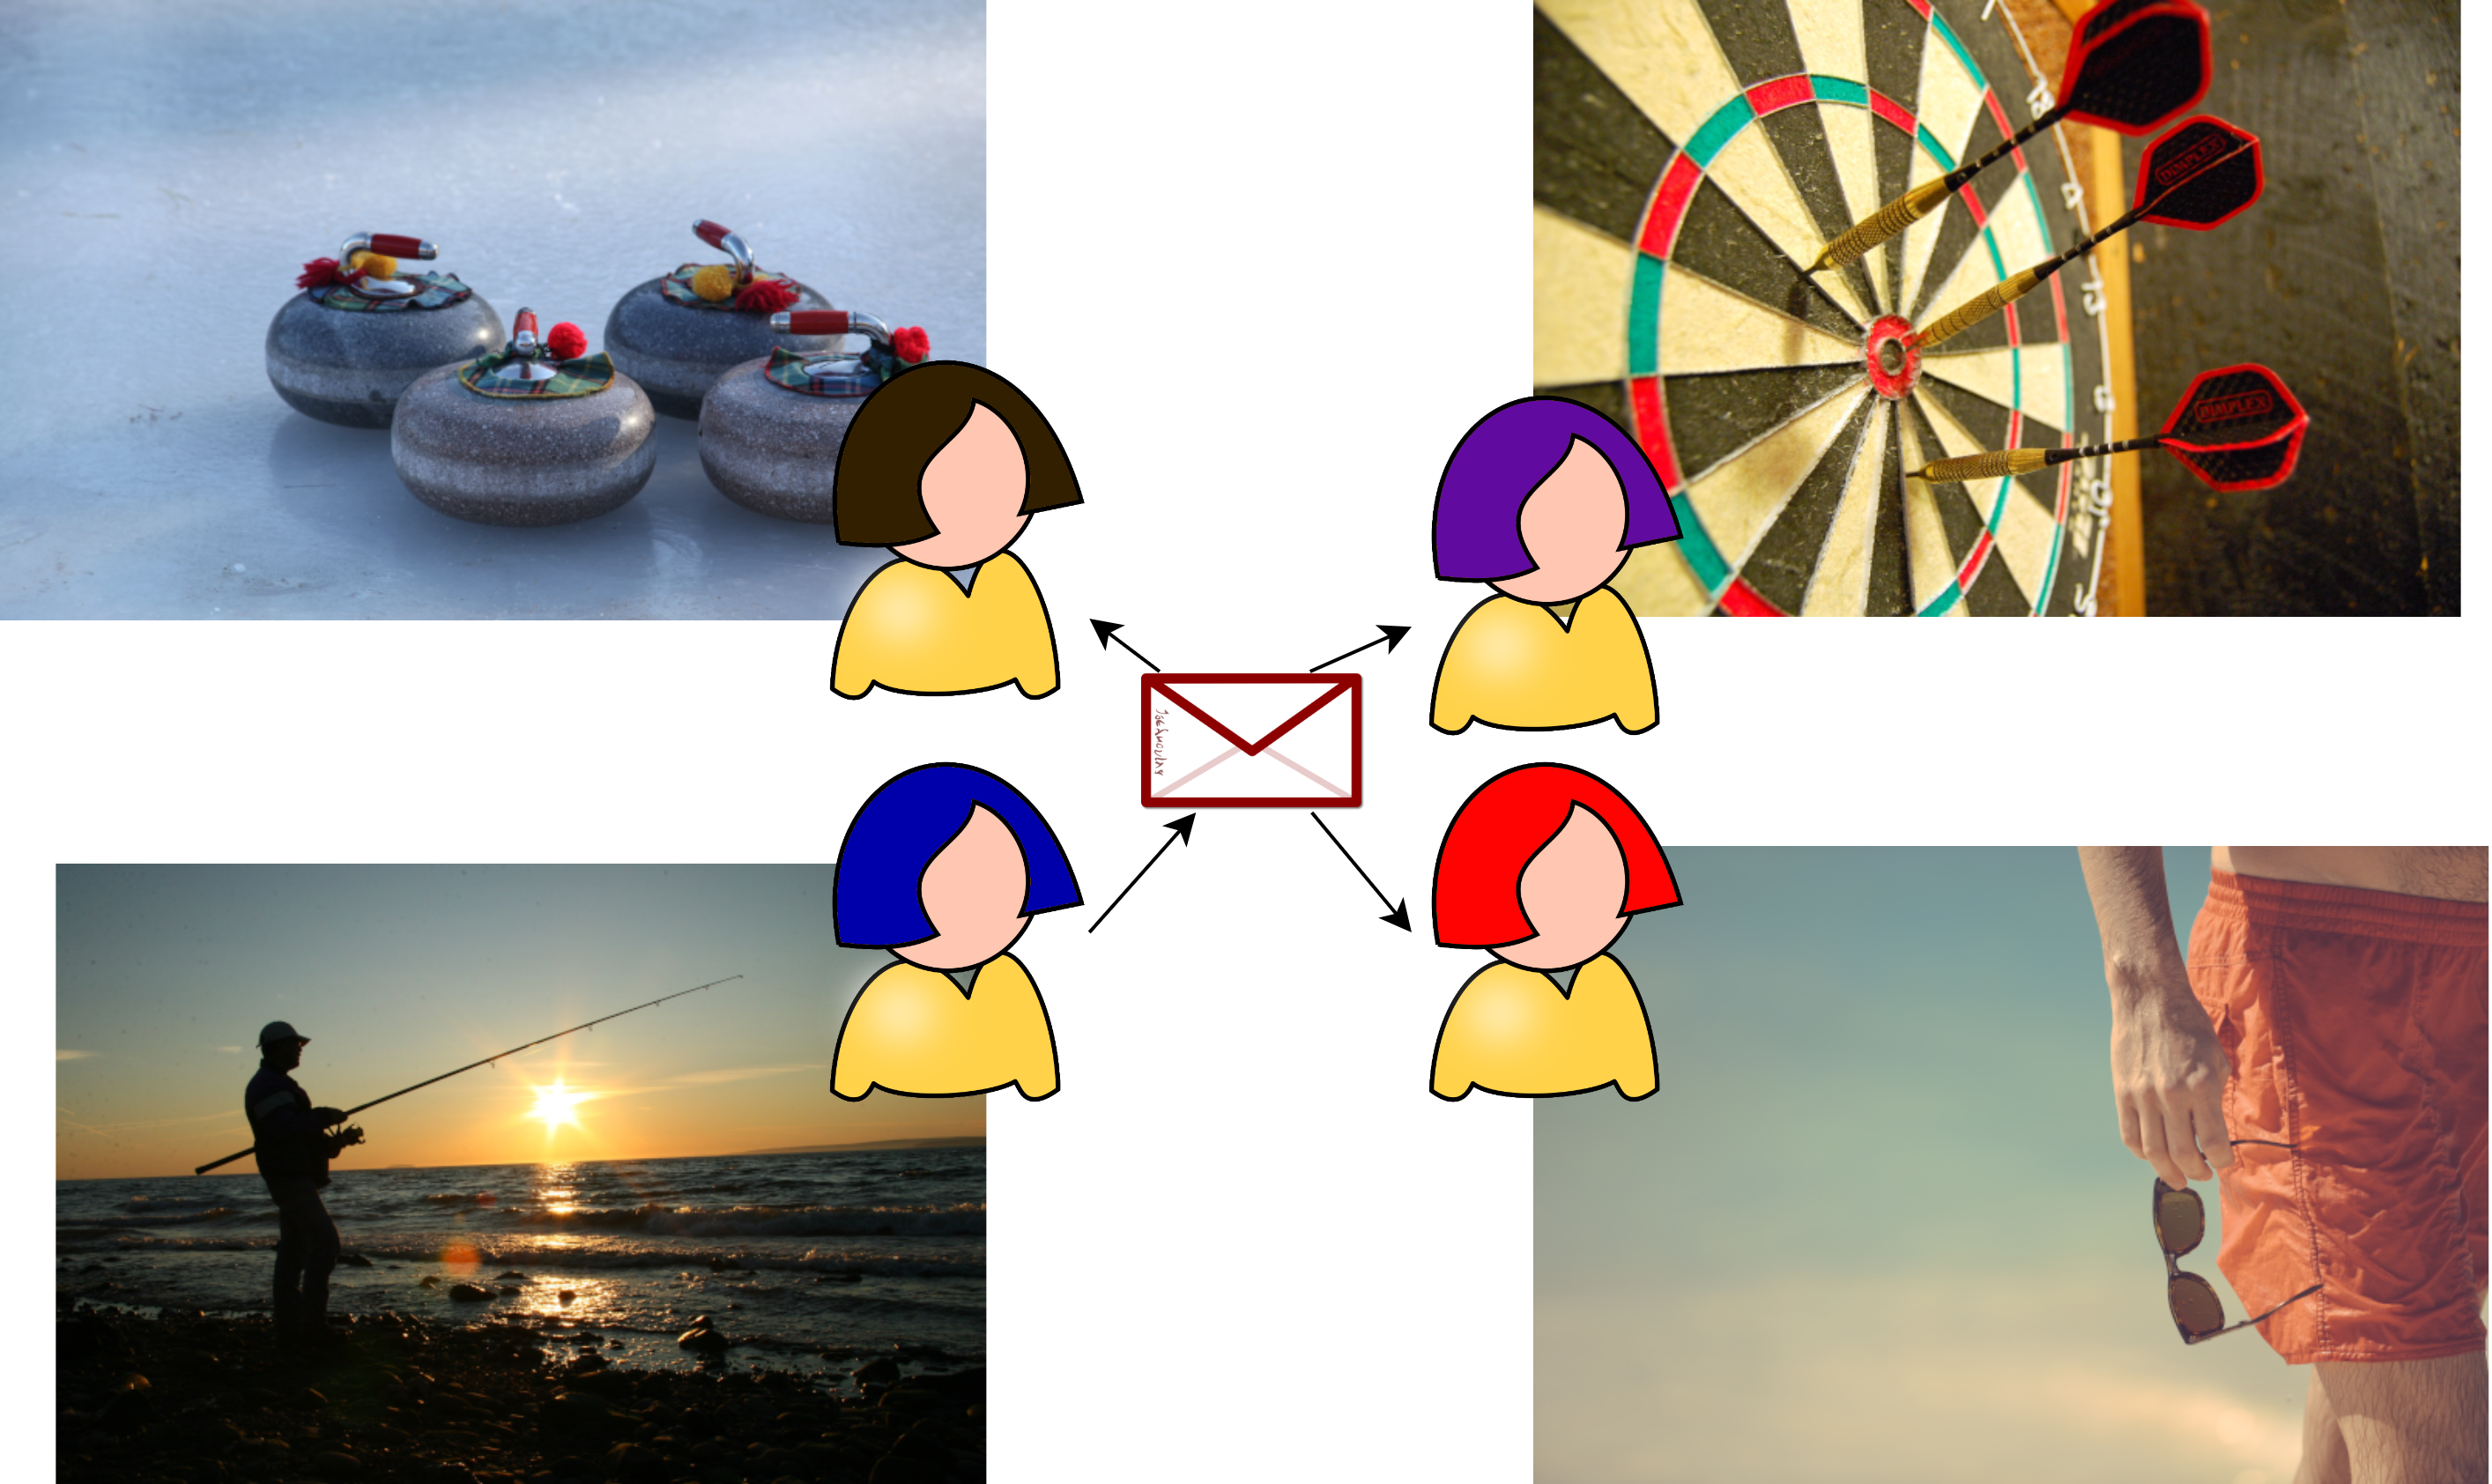
\includegraphics[width=10cm]{\imgLf/switchi.png}
  \end{center}
\end{frame}


\begin{frame}
  \frametitle{LF11c:01:::UML, Flowchart, BPMN \& (e)EPK}

  \begin{tiny}
  \parbox{.7\textwidth}{
  In der Zentrale der Sportfirma 'Switchi' arbeiten 4 Schwestern, \textbf{Anna}, \textbf{Berta}, \textbf{Charlotte} und \textbf{Dora} Bridgerton. Jede Schwester betreut eine Abteilung: Anna das \textbf{Angeln}, Berta das \textbf{Baden}, Charlotte das \textbf{Curling} und Dora \textbf{Darts}. 
  Ihre Aufgabe ist es, den Informationsaustausch zwischen den Abteilungen zu ermöglichen: 
  }\hfill\parbox{.3\textwidth}{
    \begin{center}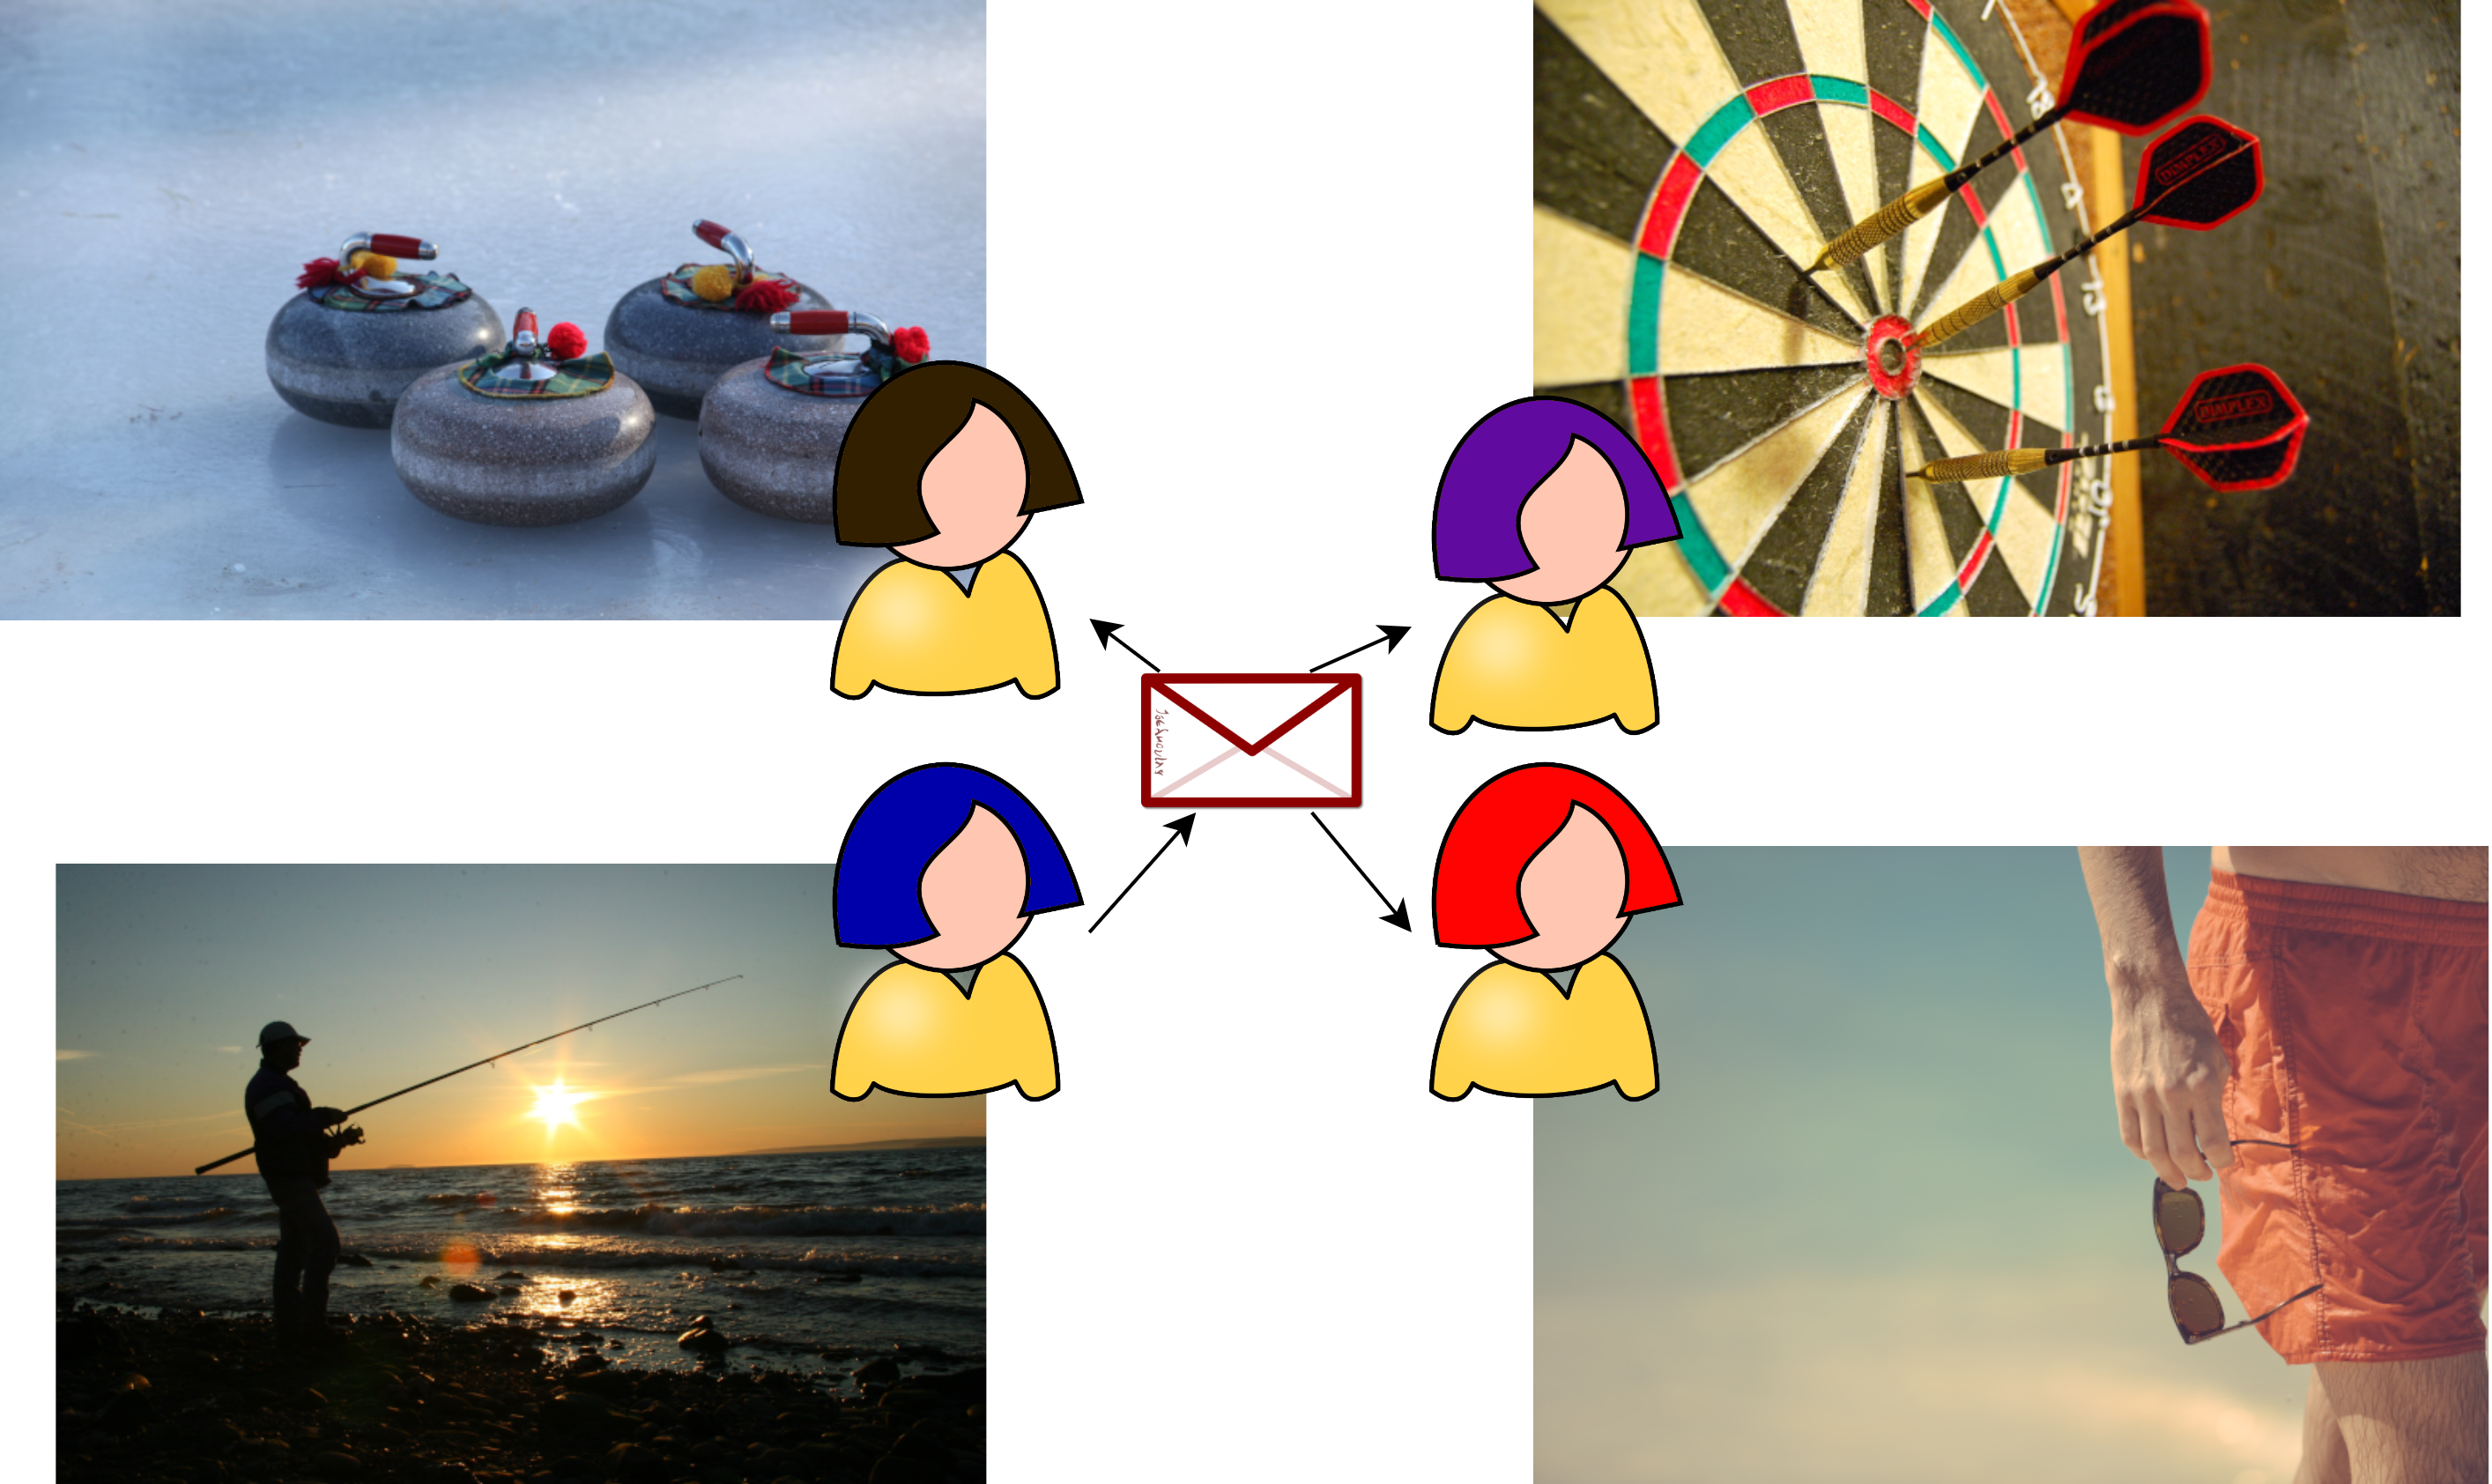
\includegraphics[width=1.1cm]{\imgLf/switchi-core.png}\end{center}
  }
  \end{tiny}

  \parbox{1\textwidth}{
  \begin{footnotesize}
  \begin{itemize}
    \item \textit{Bekommt} eine der Schwestern \textit{einen Brief} aus der Abteilung, für die sie zuständig ist, \textit{analysiert} sie den oder \textit{die Adressaten}:  
    \item Ist der Brief an alle anderen Abteilungen adressiert, \textit{läuft sie zum Kopierer}, \textit{kopiert ihn zweimal} und \textit{übergibt jeder} ihrer Schwestern \textit{einen Brief}.   
    \item Ist der Brief dagegen an eine bestimmte Abteilung adressiert, \textit{übergibt sie den Brief direkt} an die Schwester, die für diese Abteilung zuständig ist. 
    \item \textit{Reicht eine Schwester einen Brief an eine andere} Schwester, \textit{schickt diese den an die Abteilung, für die sie zuständig ist}.
  \end{itemize}
  \end{footnotesize}
  }

  \vspace{0.2cm}
  \begin{tiny}
  \parbox{1\textwidth}{
  Der Chef lässt die Abteilungen oft und überraschend in andere Zimmer ziehen. Das fördere den Teamgeist. Deshalb kennen die Abteilungen erst einmal nur ihre eigene, aktuell gerade gültige Adresse. Und sie müssen, wollen sie eine andere Abteilung kontaktieren, darum zuerst deren aktuelle Adresse ermitteln. Dazu schicken zuerst an alle Abteilungen die Frage nach der Adresse der Abteilung, mit der sie reden wollen. 
  }
  \end{tiny}

  \vspace{0.1cm}
  \begin{tiny}
    \parbox{1\textwidth}{
  Abteilungen, die mit der Frage nicht gemeint sind, \textit{ignorieren diese}. Die tatsächlich \textit{gemeinte Abteilung schickt} dagegen der anfragenden Abteilung -- sie hat deren Adresse im Absender gefunden -- \textit{als Antwort ihre eigene Adresse}. Danach können die beiden Abteilungen für eine kleine Weile \textit{direkt Nachrichten austauschen}.
    }
  \end{tiny}

\end{frame}

% This file is part of the Open Source project 'proTironeComputatri'
% (c) 2025 Karsten Reincke (https://github.com/pro-tirone-computatri/protico.ltx)
% It is distributed under the terms of the creative commons license
% CC-BY-4.0 (= https://creativecommons.org/licenses/by/4.0/)

\selectlanguage{ngerman}

\begin{frame}
  \frametitle{Stopp: Jetzt folgen Lösungsvorschläge.}
  \begin{center}
    \includegraphics[height=7.8cm]{\imgGl/stopp-wm.png}
  \end{center}
\end{frame}


\begin{frame}
  \frametitle{Umsetzungsvorschlag: BPMN Diagramm}
  \begin{center}
    \includegraphics[height=7.8cm]{\imgLf/switchi-bpmn.png}
  \end{center}
\end{frame}

\begin{frame}
  \frametitle{Umsetzungsvorschlag: EPC/EPK Diagramm}
  \begin{center}
    \includegraphics[height=7.8cm]{\imgLf/switchi-epc.png}
  \end{center}
\end{frame}

%%%%%%%%%%%%%%%%%%%%%%%%%%%%%%%%%%%%%%%%%%%
% be careful to modify the closing commands

% 1. Insert the legally necessary closure sheet
% that should be the same for each
% proTironeComputatri presentation
% This file is part of the Open Source project 'proTironeComputatri'
% (c) 2025 Karsten Reincke (https://github.com/pro-tirone-computatri/protico.ltx)
% It is distributed under the terms of the creative commons license
% CC-BY-4.0 (= https://creativecommons.org/licenses/by/4.0/)
\selectlanguage{ngerman}
\begin{frame}
  \frametitle{Abschluss}
    
  \vspace{0.2cm}
  \begin{center}
    Herzlichen Dank für Ihre Aufmerksamkeit!
  \end{center}

  \vspace{0.2cm}
  \begin{center}
    \includegraphics[height=2cm]{\imgGl/logo-protirone.png} \hspace{0.2cm}
    \href{https://de.wikipedia.org/wiki/Open\_Educational\_Resources}{\includegraphics[height=2cm]{\imgGl/logo-oer.png}}

  \end{center}
    
  \begin{footnotesize}
    Diese Präsentation gehört zum Open-Source-Projekt
    \textrm{\textit{proTironeComputatri}}\footnote{\tiny{$\rightarrow$ 
    \href{https://github.com/pro-tirone-computatri/}{https://github.com/pro-tirone-computatri/}}},
    initiiert v. Karsten Reincke, Hohenahr\footnote{\tiny{$\rightarrow$ 
    \href{https://github.com/pro-tirone-computatri/protico.ltx/CONTRIBUTORS.md}
    {https://github.com/pro-tirone-computatri/protico.ltx/CONTRIBUTORS.md}}}. Die Unterrichtseinheiten stehen unter den 
    Bedingungen der \href{https://creativecommons.org/licenses/by/4.0/}{CC-BY-4.0}-Lizenz zur freien Verfügung. 
    Die Quellen dazu finden Sie unter \textit{protico.ltx}\footnote{\tiny{$\rightarrow$
    \href{https://github.com/pro-tirone-computatri/protico.ltx}{https://github.com/pro-tirone-computatri/protico.ltx}}}.
  \end{footnotesize}
    
\end{frame}

% 2. hide the logo
\logo{}
\newpage

% 3. insert the image credit list
% This file is part of the Open Source project 'proTironeComputatri'
% (c) 2025 Karsten Reincke (https://github.com/pro-tirone-computatri/protico.ltx)
% It is distributed under the terms of the creative commons license
% CC-BY-4.0 (= https://creativecommons.org/licenses/by/4.0/)


% requires an locally computed file inc-image-list.tex
% computation command is included in the makefiles
\newpage
\section{Bildnachweise}
\noindent\rule{\linewidth}{0.4pt}

\begin{small}Bildnachweise\end{small}

\vspace{0.22cm}
\begin{tiny}
 \begin{itemize}
   \item \includegraphics[height=8pt]{\imgGl/logo-protirone.png} von Karsten Reincke. \href{https://github.com/pro-tirone-computatri/protico.ltx/blob/main/LICENSING.md}{Lizenziert} unter \href{https://github.com/pro-tirone-computatri/protico.ltx/blob/main/LICENSING.md}{proTirone-Logo-License}. Bereitgestellt auf \href{https://github.com/pro-tirone-computatri/protico.ltx/}{github}. (may only be used as logo for proTirone)
   \item \includegraphics[height=8pt]{\imgGl/split-680866-pxh.png} von anonymous. \href{https://pxhere.com/en/photo/680866}{Lizenziert} unter \href{https://creativecommons.org/publicdomain/zero/1.0/}{CC0}. Bereitgestellt auf \href{https://pxhere.com/en/photo/680866}{Pxhere:680866}.
\end{itemize}

\end{tiny}


% 4. insert the liteature hints 
%% This file is part of the Open Source project 'proTironeComputatri'
% (c) 2025 Karsten Reincke (https://github.com/pro-tirone-computatri/protico.ltx)
% It is distributed under the terms of the creative commons license
% CC-BY-4.0 (= https://creativecommons.org/licenses/by/4.0/)

\newpage
\section{Literaturliste}
\noindent\rule{\linewidth}{0.4pt}

\begin{small}Literaturliste\end{small}

\vspace{0.22cm}
\printbibliography
\end{document}

